% LaTeX Template for short student reports.
% Citations should be in bibtex format and go in references.bib
\documentclass[a4paper, 11pt]{article}
\usepackage[top=3cm, bottom=3cm, left = 2cm, right = 2cm]{geometry} 
\geometry{a4paper} 
\usepackage[utf8]{inputenc}
\usepackage{textcomp}
\usepackage{graphicx} 
\usepackage{amsmath,amssymb}  
\usepackage{bm}  
\usepackage[pdftex,bookmarks,breaklinks]{hyperref}  
%\hypersetup{linkcolor=black,citecolor=black,filecolor=black,urlcolor=black} % black links, for printed output
\usepackage{memhfixc} 
\usepackage{pdfsync}  
\usepackage{fancyhdr}
\pagestyle{fancy}
\usepackage{algorithm}
\usepackage{algpseudocode}

\title{Data Structures II (CS-201) Project Report \\ Dynamic Trees for optimized Network Flow algorithms}
\author{Musab - 07811, Sara Baloch - 08586, Meesum Abbas - 08056, Rameez Wasif - 08479}
%\date{}

\begin{document}
\maketitle
\pagebreak
\tableofcontents
\pagebreak

\section{Abstract}
We implemented an optimized data structure presented in a research paper for the problem of Dynamic Trees. We visualise its operations and empirically evaluate whether its operations match the theoretical bounds, particularly in the problem of finding the max flow in a network where it is deemed to be $O(nm\log{n})$.

\pagebreak

\section{Intro}

For our project, we decided to implement a data structure and visualise its operations based off the paper \emph{"A Data Structure for Dynamic Trees"} \cite{DynamicTrees} by Dr Sleator and Dr Tarjan. This data structure provides a solution for the Dynamic Trees problem, different from the obvious solution, in order to optimize some operations, at the cost of slowing down some others. While it may seem like a harsh tradeoff, this optimization allows the implementation of a max-flow algorithm with time-complexity $O(mn\log{n})$ as opposed to a time-bound of $O(n^2m)$ of Dinit's original algorithm and the previously best $O(nm(\log{n})^2)$ for sparse graphs by Galil and Naamad. The max-flow problem is crucial in network routing, transportation and logistics. Therefore, this data structure is incredibly valuable for real-world problems where the order of data is large and these asymptotic improvements become equivalent to days of computing power.
\\
In our report, in section 3 we explore the Data Structure, sharing our own key insights. In section 4, we review the functionality of our implementation and share visualisations of the tree and some of its operations. In section 5, we take a look at Network Flow algorithms. In section 6, we test our data structure and carry out analysis on its computation time and accuracy. In section 7, we offer our review on the data structure and the project overall.

\pagebreak

\section{Understanding the Data Structure}
First, we aim to comprehend the paper's essence. In simple terms, our goal is to represent a tree that undergoes many changes - a Dynamic Tree - and efficiently update it. While representing the tree in its raw form might suffice for certain tasks, offering a time complexity $O(1)$ for some operations, for others, it could incur a time complexity of $O(n)$, which is undesirable. Is there a middle ground, a workaround?

Operations on a tree are dependent on its height. So the simple solution is to balance the tree. But the problem is, you actually want the original tree - with its root and its connections, so you can’t balance it. So the data structure has an external representation and an internal representation, each with their own functions. Putting all of this together gives us around 4 levels of abstraction.

We begin by assuming all nodes are unconnected and define the following eight operations of the Dynamic Tree, i.e. the upper most interface (pseudocode available in the paper):
\begin{enumerate}
    \item \texttt{parent(v)}: Obtain the parent of node \(v\) (return null if no parent).
    \item \texttt{root(v)}: Retrieve the root of the tree.
    \item \texttt{cost(v)}: Access the cost of an edge between a node and its parent (\(v\) must not be a tree root).
    \item \texttt{mincost(v)}: Identify the vertex \(w\) between \(v\) and the $root(v)$ with the minimum cost. In case of a tie, select the vertex closest to the root (\(v\) must not be a tree root).
    \item \texttt{update(v, x)}: Increment the cost of all edges in the path from \(v\) to $root(v)$ by \(x\).
    \item \texttt{link(v, w, x)}: Establish an edge (\(v, w\))—with \(w\) becoming the parent—having a cost of \(x\), where \(v\) is a tree root. This operaton combines their respective trees.
    \item \texttt{cut(v)}: Sever the tree containing \(v\) by breaking the edge between \(v\) and its parent (\(v\) must not be a tree root).
    \item \texttt{evert(v)}: Modify the tree containing \(v\) such that \(v\) becomes the root.
\end{enumerate}

The paper explores an option to represent the tree using an alternative data structure commonly called the ST Link-Cut Tree (when referring to Dynamic Trees, we will be referring to this implementation of the Dynamic Tree unless otherwise specified). Specifically, it separates the tree into two parts. Some edges are grouped together to form different paths, while the remaining edges are stored in a map for efficient access. Consequently, when modifications to multiple edges within a tree are required, operations are applied on the overarching path containing those edges, which proves quicker than altering each edge individually. The remaining edges are modified as normal.

\begin{table}[h]
\centering
\caption{Comparison of Operations in Implementations of Dynamic Trees}
\label{table:comparison}
\begin{tabular}{|c|c|c|}
\hline
\textbf{Operation} & \textbf{Generic Tree Representation} & \textbf{ST Link-Cut Tree Representation} \\
\hline
parent(v) & $O(1)$ & $O(\log n)$ \\
\hline
root(v) & $O(n)$ & $O(\log n)$ \\
\hline
cost(v) & $O(1)$ & $O(\log n)$ \\
\hline
mincost(v) & $O(n)$ & $O(\log n)$ \\
\hline
update(v, x) & $O(n)$ & $O(\log n)$ \\
\hline
link(v, w, x) & $O(1)$ & $O(\log n)$ \\
\hline
cut(v) & $O(1)$ & $O(\log n)$ \\
\hline
evert(v) & $O(n)$ & $O(\log n)$ \\
\hline
\end{tabular}
\end{table}

The edges in the map are represented as dashed edges in the diagrams, while the edges in paths are depicted as bold edges. Additionally, it's important to note that a vertex can only belong to one path. Moreover, a path always ascends, with its head being the lowest node in the path and its tail being the highest node.

\begin{figure}
    \centering
    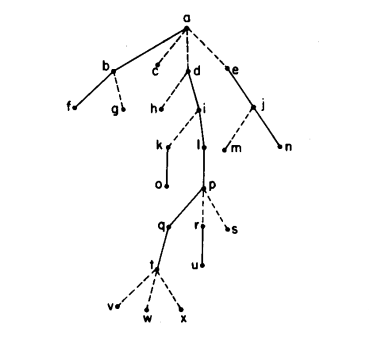
\includegraphics[width=0.5\textwidth]{img/diagrams/dyn_tree.png}
    \caption{An example of a dynamic tree. The bold edges represent paths while the dashed edges are stored in maps. (source: paper)}
    \label{fig:1}
\end{figure}

Descending one layer of abstraction, we encounter the \texttt{splice} and \texttt{expose} functions (pseudocode provided in the paper). 

The \texttt{splice(v)} function extends a bold path upwards by permitting a bridge over one dashed edge, making it bold. However, in making this connection bold, the previous connection of the node to its other children becomes dashed.

\begin{figure}
    \centering
    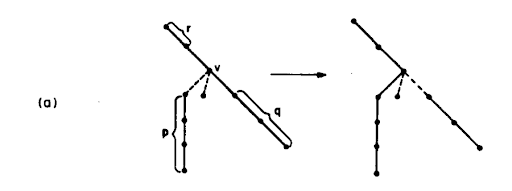
\includegraphics[width=0.5\textwidth]{img/diagrams/splice.png}
    \caption{The effect of a splice operation. The connection of $v$ to $p$ becomes bold while it's other downward connection (with $q$ becomes dashed) (source: paper)}
    \label{fig:2}
\end{figure}

The \texttt{expose(v)} function connects a node all the way to the root via a bold path and makes and downward connections from a node dashed. Essentially, it applies splice over and over again until we reach the root. It also makes my children dashed.

\begin{figure}
    \centering
    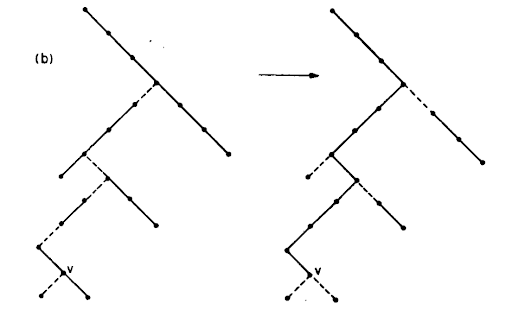
\includegraphics[width=0.5\textwidth]{img/diagrams/expose.png}
    \caption{The effect of an expose operation.  (source: paper)}
    \label{fig:3}
\end{figure}

Moving down another layer of abstraction, let’s now look at the path. It is stored as a full tree, where each of the non-leaf nodes (internal + root) represent an edge. Moreover, its subtree represents a subpath. The leaves/external nodes represent the vertices in the path. Figure \ref{fig:4}. is handy.

\begin{figure}
    \centering
    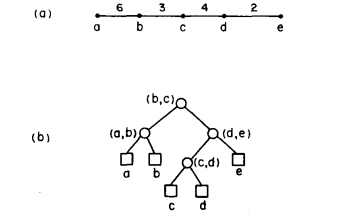
\includegraphics[width=0.5\textwidth]{img/diagrams/internal_paths.png}
    \caption{A path and its internal representation.  (source: paper)}
    \label{fig:4}
\end{figure}

Moreover, if we do an inorder traversal of the path, that gives us a path from head to tail, or if talking about our original tree, it’s a path moving upwards.

Before we look at each of these nodes, let’s clarify two important terms related to costs of edges:

\begin{itemize}
    \item \texttt{Grosscost}: Cost of the edge represented by a node.
    \item \texttt{Grossmin}: Least cost of all the edges in the path represented by the subtree of a node.
\end{itemize}

\begin{figure}
    \centering
    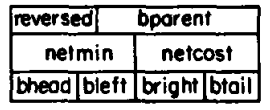
\includegraphics[width=0.5\textwidth]{img/diagrams/internal_node.png}
    \caption{An internal node's contents.  (source: paper)}
    \label{fig:5}
\end{figure}

Each node has many aspects. Let’s take a look at each of these:
\begin{itemize}
    \item \texttt{Reversed}: Denotes the reversal state of the path represented by the node's subtree. If a node is reversed, its left child is its right child and vice versa + its head is its tail and vice versa. \\ \textbf{Note}: The actual reversal state of a node is determined by counting the number of reversal states from the node to root. If odd then the node/path is reversed, if even, then all the reversals cancel out and the node/path is not reversed.
    \item \texttt{Bparent}: Node's parent in the tree.
    \item \texttt{Netmin}: The difference between the mincost edge in the path represented by the node's subtree and the mincost edge of the path represented by the node's parent’s subtree $\rightarrow$ \texttt{grossmin(v)} if $v$ is root else \texttt{grossmin(v)} - \texttt{grossmin(parent(v))}. \\ \textbf{Note}: The grossmin of a node can be found by summing up the netmin from the node to the root of the path. In a sense, it’s similar to prefix sums.
    \item \texttt{Netcost}: How much greater is the cost of the edge represented by this node as compared to the mincost of the subtree represented by this node $\rightarrow$ \texttt{grosscost(v)} - \texttt{grossmin(v)}.
    \\ \textbf{Note}: If we know the grossmin of a node, we can get its cost i.e. the cost of the edge represented by this node, by summing up grossmin and netcost.
    \item \texttt{Bhead}: The head of the path represented by the node's subtree.
    \item \texttt{Bleft}: The left child of the node in the binary tree.
    \item \texttt{Bright}: The right child of the node in the binary tree.
    \item \texttt{Btail}: The tail of the path represented by the node's subtree.
\end{itemize}

Note that some of these properties are not relevant for a leaf node, e.g. \texttt{netmin} and \texttt{netcost}. \\

\begin{figure}
    \centering
    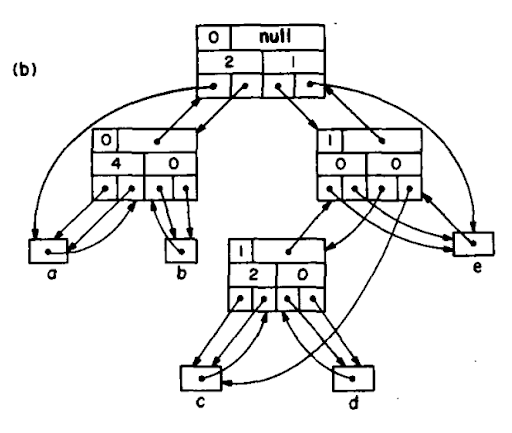
\includegraphics[width=0.5\textwidth]{img/diagrams/internal_tree.png}
    \caption{An internal tree for the path in Figure 4. with each node's attributes shown.  (source: paper)}
    \label{fig:6}
\end{figure}

We use 11 operations to work on these paths (explanations for implementation for the first 9 operations are provided in the paper) - note that \texttt{v} refers to a vertex and \texttt{p} to a path:

\begin{enumerate}
    \item \texttt{path(v)} - Find the node identifying the path of a vertex, i.e., the root of the tree (simply traverse upwards from the vertex node until unable to proceed).
    \item \texttt{head(p)} - Find the first node in the path, considering reversal states (access the \texttt{head} of the path if the path isn’t reversed, otherwise access the \texttt{tail}).
    \item \texttt{tail(p)} - Symmetric to \texttt{head}.
    \item \texttt{before(v)} - Find the vertex just before \(v\) in the bold path (ascend the path until the current node is a right child of some parent node, then access this parent node's left child and obtain its \texttt{tail}).
    \item \texttt{after(v)} - Symmetric to \texttt{before}.
    \item \texttt{pcost(v)} - Find the cost of the edge \((v, \texttt{after}(v))\) (traverse upwards until the current node is a left child of some parent node, similar to \texttt{after}. This node represents the edge between \((v, \texttt{after}(v))\). Determine its cost by computing \texttt{grossmin} (method detailed earlier) and adding it to \texttt{netcost}).
    \item \texttt{pmincost(p)} - Find the cost of the smallest edge in the path. In case of a tie, choose the one closest to the tail of the path. \\ \textbf{Note}: the description of this has a slight error in the paper, a complete revised description is provided in the Appendix note 1.
    \item \texttt{pupdate(p, x)} - Add \(x\) to the cost of all edges in the path (add \(x\) to \texttt{netmin} of \(p\)).
    \item \texttt{reverse(p)} - Reverse the path (change reverse bit of \(p\)).
    \item \texttt{concatenate(p, q, x)} - Join two paths using an edge of cost \(x\).
    \item \texttt{split(v)} - Break the path into the path before \(v\) and the path after \(v\).
\end{enumerate}

Note that for each of these functions, we have to be mindful of reversal states - for example, in the stopping conditions for \texttt{before}, where we are looking for a node where \(v\) is a right child. If the node is reversed, then we will check if \(v\) is its left child.

\texttt{Concatenate} and \texttt{Split} are special because they actually modify the path, while the others simply traverse it and access/modify some node data. Since they manipulate the structure of the path, we need a way to optimize how these changes occur, ensuring future operations can continue to be performed efficiently.

However, another barrier we face is that such an important function doesn’t actually have much description in the paper… at least not this one.

Initially, we started with a rather simplistic implementation:

\begin{itemize}
    \item For \texttt{concatenate}, simply create a new node linked to the root of both paths.
    \item For \texttt{split}, note that the parent in the path tree for a vertex is an edge connected to it. Rotate this edge upwards until it's at the top of the tree. Once it's at the top, delete this node and update its immediate children if necessary. Repeat this process a second time if needed, as a node can have two edges connected to it (in and out).
\end{itemize}

This implementation, while functional, is not optimal. For a random sequence of operations, this is just fine and actually faster than what's targeted in the paper. However, there exists some sequence of \(m\) operations where our time complexity approaches \(O(mn)\), where \(m\) is the number of nodes in the tree. Particularly, this happens in the sequence of steps that links nodes in the order $1, 2, 3,\ldots, n$ and then cuts it as $1, 2, 3, \ldots, n$. This isn't ideal. Luckily, there is an optimization we can still do to cut this down to \(O(m \log n)\).

To understand how these optimizations take place, we have to refer to Sleator, Tarjan and Bent's paper on \emph{“Biased Search Trees.”} \cite{BiasedSTrees} Here, we basically try to keep more frequently required nodes higher up in the tree, while less frequently accessed nodes are kept lower down. Through some analysis, Sleator and Tarjan highlight that this setup actually amortizes the cost to \(O(\log n)\), which is exactly what we need to speed up the data structure.

\texttt{Concatenate} and \texttt{Split} are mentioned in this other paper, along with one of their helper functions - \texttt{tilt} (left and right).

However, these operations are built on top of a 4th level of abstraction (partly referenced in our description of \texttt{concatenate} and \texttt{split}). This includes the functions:

\begin{itemize}
    \item \texttt{construct(u, v, x)} - Given the roots \(v, w\) of two trees and a real value \(x\), combine the trees by creating a new node with left child \(v\) and right child \(w\) and \texttt{grosscost} \(x\).
    \item \texttt{destroy(u)} - Given a root \(u\) of a non-trivial tree, delete \(u\), returning \([v, w, x]\) where \(v\) is its left child, \(w\) is its right child, and \(x\) is the cost of the edge represented by \(u\). Note that since our binary tree is always full, both children will exist for a non-trivial tree.
    \item \texttt{rotateleft(v)} - Perform a single left rotation at node \(v\). Node \(v\) must have an internal right child.
    \item \texttt{rotateright(v)} - Perform a single right rotation at node \(v\). Node \(v\) must have an internal left child.
\end{itemize}

For the last two operations, we opted for a single option \texttt{rotate(v)}, which takes the child of the node being rotated and determines the type of rotation based on whether it is a left child or a right child.

Generally, these operations are standard tree operations, but in our case, we have some messy attributes to be careful with—namely cost and reversal state. We will go over solutions to these operation by operation.
\begin{enumerate}
\item \texttt{construct(u, v, x)}:
\begin{itemize}
    \item \textbf{Cost}: The \texttt{netmin} of the new node is supposed to represent the combined \texttt{grossmin} of \(u\), \(v\), and \(x\), so we just consider the minimum of \(x\), \texttt{netmin(u)}, \texttt{netmin(v)} since \(u\) and \(v\) have no parents and therefore their \texttt{netmin} is their \texttt{grossmin}. \(x\) is the \texttt{grosscost} of the new node so we can determine the \texttt{netcost} by subtracting \texttt{grossmin} from \(x\). Also note that the children of this new node now have parents so their \texttt{netmin} will be updated, particularly, their \texttt{netmin} -= the new node’s \texttt{netmin}. Their \texttt{netcost} is not updated as \texttt{netcost} depends upon \texttt{grosscost} and \texttt{grossmin} which only refers to their own subtrees, thus adding a node above has no effect.
    \item \textbf{Reversal}: Set the reversed state of new node to 0.
\end{itemize}

\item \texttt{destroy(u)}:
\begin{itemize}
    \item \textbf{Cost}: Since \(u\)'s children will no longer have parents, we must add back \(u\)'s \texttt{grossmin} (same as $u$'s \texttt{netmin}) to their \texttt{netmin}.
    \item \textbf{Reversal}: If $u$ is reversed, then flip the reversal state of both it's children before deleting.
\end{itemize}

\item \texttt{rotate(v)}:
\begin{itemize}
    \item \textbf{Cost}: Let \(u\) be the parent of \(v\), \(s\) be the sibling of \(v\), \(c\) be the child of \(v\) that stays \(v\)’s child, and \(x\) be the child of \(v\) that becomes \(u\)’s child.
    \begin{itemize}
        \item \textbf{Case 1}: The \texttt{grossmin} of \(u\) was in \(v\)’s subtree:
        \begin{itemize}
            \item \(v\)’s \texttt{netmin} becomes \(u\)’s previous \texttt{netmin} since it has \(u\)’s previous \texttt{grossmin} and \(u\)’s previous parent. \(v\)’s \texttt{netcost} is unchanged since its \texttt{grossmin} is unchanged.
            \item \(c\) is unchanged since its parent’s \texttt{grossmin} is unchanged and its subtree is unchanged.
            \item \(u\)’s \texttt{netmin} becomes the least out of its previous \texttt{netcost} and its new children’s (\(s\), \(x\)) previous \texttt{netmin}, because its children’s previous \texttt{netmin} were with respect to the \texttt{grossmin} of \(u\) which is now the \texttt{grossmin} of \(v\). And its \texttt{netcost} was how much more it was from its previous \texttt{grossmin} which is now the \texttt{grossmin} of \(v\). \(u\)’s \texttt{netcost} is reduced by its \texttt{netmin} as \(u\)’s \texttt{grossmin} has increased by \texttt{netmin}.
            \item For \(s/x\), \texttt{netmin} is reduced by \(u\)’s new \texttt{netmin} as \(u\) now acts like an intermediate between \(s/x\) and the actual smallest edge—keep in mind the prefix sum type property. \texttt{Netcost} unchanged as subtree unchanged.
        \end{itemize}
        \item \textbf{Case 2}: The \texttt{grossmin} of \(u\) was not in \(v\)’s subtree:
        \begin{itemize}
            \item \(v\)’s \texttt{netmin} becomes \(u\)’s previous \texttt{netmin} since it has \(u\)’s previous \texttt{grossmin} (due to having \(u\)’s previous subtree) and \(u\)’s previous parent. \(v\)’s \texttt{netcost} increases by \texttt{netmin} since its \texttt{grossmin} has decreased by as much.
            \item \(c\)’s \texttt{netmin} is increased by \(v\)’s new \texttt{netmin} as \(v\)’s \texttt{grossmin} has decreased by as much. Its \texttt{netcost} is unchanged since its subtree is unchanged.
            \item \(u\)’s \texttt{netmin} becomes the least out of its previous \texttt{netcost} and its new children’s (\(s\), \(x\)) previous \texttt{netmin}, because its children’s previous \texttt{netmin} were with respect to the \texttt{grossmin} of \(u\) which is now the \texttt{grossmin} of \(v\). And its \texttt{netcost} remains unchanged as it has the smallest edge and so its \texttt{grossmin} is unchanged.
            \item For \(s\), \texttt{netmin} is reduced by \(u\)’s new \texttt{netmin} as \(u\) now acts like an intermediate between \(s\) and the actual smallest edge—keep in mind the prefix sum type property. \texttt{Netcost} unchanged as subtree unchanged.
            \item For \(x\), \texttt{netmin} increases by the original \texttt{netmin} of \(v\) as \(v\) used to act like an intermediate between \(x\) and the actual smallest edge—keep in mind the prefix sum type property. \texttt{Netcost} unchanged as subtree unchanged.
        \end{itemize}
    \end{itemize}
    \item \textbf{Reversal}: If the reversal state of \(v\) is 1, we should resolve this before rotating, i.e., swap $v$'s left and right children as well as itst head and tail and flip its reversal state. If $v$'s parent is reversed, that means the path in its subtree is reversed. However, after $v$ is rotated, its subtree will have all the same nodes it's former parent's subtree had. So $v$ just takes its former parent's reversal state and $v$'s former parent takes a reversal state of 0.
\end{itemize}
\end{enumerate}
There’s one last thing to look at before we’re done with our data structure. And that is ranks and weights for optimization. 

The paper states that the rank of a node should be the logarithm (base 2) of its weight.

Moreover, it describes weight for leaf nodes to be:
\[
\text{wt}(v) = 
\begin{cases} 
\text{size}(v) & \text{if no solid edge enters } v; \\
\text{size}(v) - \text{size}(w) & \text{if the solid edge } (w, v) \text{ enters } v 
\end{cases}
\]
where \(\text{size}(v)\) refers to the number of nodes in the subtree of \(v\).

Moreover, the weight of non-leaf nodes becomes the sum of the weight of its immediate children, which is also the same as the sum of the weight of all leaf nodes in its subtree.

This leads to changes in \texttt{construct}, \texttt{rotate}, \texttt{splice}, and \texttt{expose}, and it also requires that we initialize our nodes with a weight of 1 as all nodes are initially unconnected.

The changes in \texttt{construct} and \texttt{rotate} are trivial—the weight of a new node is the sum of the weights of its children. For weight after rotating a node \(v\), we can determine its original parent \(u\)'s weight by summing up the weight of its children. After doing this, we can update the weight of \(v\) by summing up the weight of its children.

The changes in \texttt{splice} and \texttt{expose} are detailed in the paper (pseudocode); however, it misses one key detail in \texttt{expose}, highlighted in Appendix note 2.

With these changes implemented, our data structure is complete and optimized.


\pagebreak

\section{Testing our Implementation}

Let us now walk through some examples of operations on the data structure and our visualizations of both the internal state and the actual tree.

For the actual tree, the labels in the node indicate the vertex, while the edges represent the cost of edges.

In the internal tree, the leaves are round and their labels indicate the vertex they represent. The non-leaf nodes are box-shaped, and their label represents the edge they refer to, e.g., (2, 1) indicates the edge (2, 1). Moreover, a * on a node indicates that it is reversed, so (2, 4)* means this node is reversed. The bold edges represent left and right children pointers, labelled as \texttt{l} and \texttt{r} respectively, while dashed edges are used for head and tail pointers, labelled as \texttt{h} and \texttt{t} respectively. The value at the top-left of a node represents its rank, which is used in balancing the internal tree.

For the first example, assume that we start with 3 nodes with no connections as in Figure \ref{fig:7}. We perform the operation \texttt{link(2, 1, 5)} making 1 the parent of 2 through an edge of cost 5 (Figure \ref{fig:8}). Now we perform the operation \texttt{link(3, 2, 4)}. Note that in Figure \ref{fig:9}, the \texttt{l} label is on an edge going to the right, while the \texttt{r} label is on the edge going left. This is a limitation in our visualization. However, if we just focus on the label names, we can see that if we carry out an inorder traversal on the nodes, we get the bold path of the actual tree from bottom to top.

\begin{figure}[h]
\centering
\begin{tabular}{cc}
  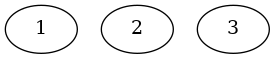
\includegraphics[width=0.5\textwidth]{img/visualisations/test1/1.png} & 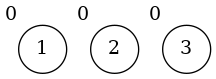
\includegraphics[width=0.5\textwidth]{img/visualisations/test1/i1.png} \\
  Actual tree & Internal tree \\
\end{tabular}
\caption{Initial tree of 3 nodes}
\label{fig:7}
\end{figure}

\begin{figure}[h]
\centering
\begin{tabular}{cc}
  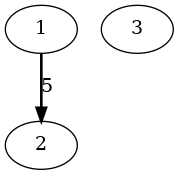
\includegraphics[width=0.3\textwidth]{img/visualisations/test1/2.png} & 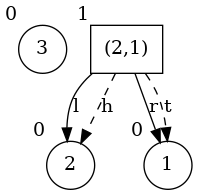
\includegraphics[width=0.3\textwidth]{img/visualisations/test1/i2.png} \\
  Actual tree & Internal tree \\
\end{tabular}
\caption{After \texttt{link(2, 1, 5)}}
\label{fig:8}
\end{figure}

\begin{figure}[h]
\centering
\begin{tabular}{cc}
  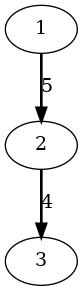
\includegraphics[width=0.1\textwidth]{img/visualisations/test1/3.png} & 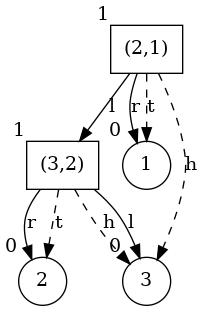
\includegraphics[width=0.25\textwidth]{img/visualisations/test1/i3.png} \\
  Actual tree & Internal tree \\
\end{tabular}
\caption{After \texttt{link(3, 2, 4)}}
\label{fig:9}
\end{figure}

\pagebreak

Let us now consider a larger example now. Consider the tree in Figure \ref{fig:10} as our initial tree. We consider separately the following operations on this tree:
\begin{itemize}
    \item \texttt{evert(4)} (Figure \ref{fig:11})
    \item \texttt{cut(2)} (Figure \ref{fig:12})
    \item \texttt{update(10, 2)} (Figure \ref{fig:13})
\end{itemize}

\begin{figure}[H]
\centering
\begin{tabular}{cc}
  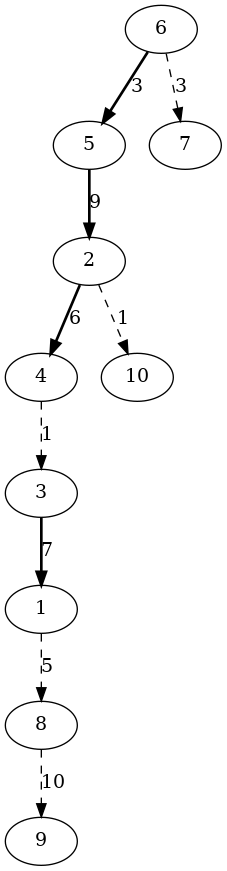
\includegraphics[width=0.25\textwidth]{img/visualisations/test2/0.png} & 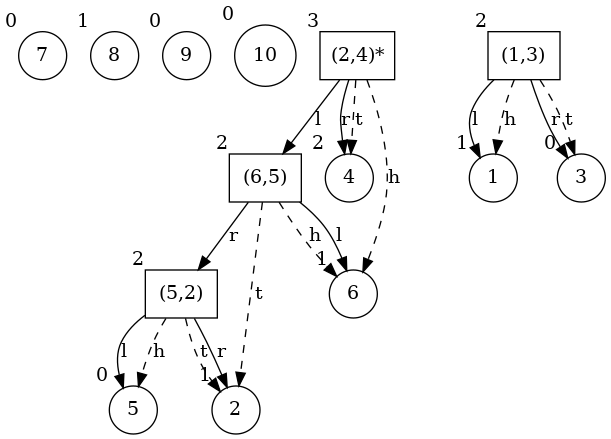
\includegraphics[width=0.7\textwidth]{img/visualisations/test2/i0.png} \\
  Actual tree & Internal tree \\
\end{tabular}
\caption{Sample Tree}
\label{fig:10}
\end{figure}

\begin{figure}[H]
\centering
\begin{tabular}{cc}
  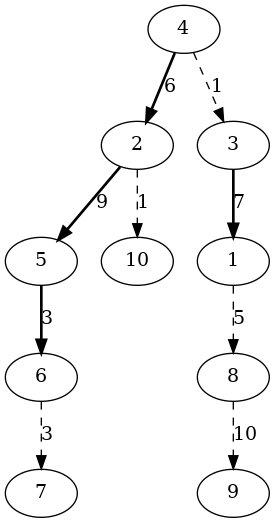
\includegraphics[width=0.3\textwidth]{img/visualisations/test2/evert.png} & 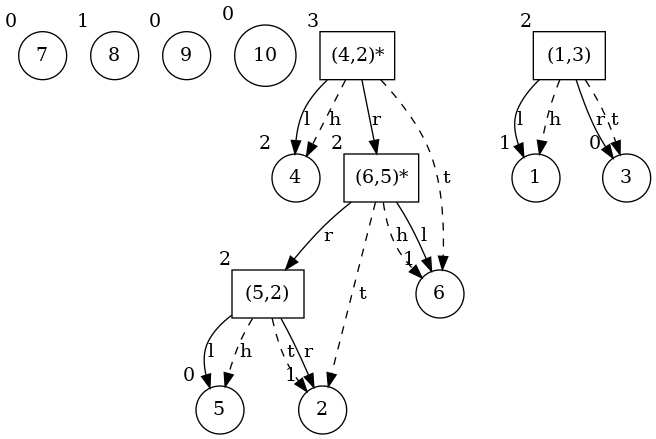
\includegraphics[width=0.6\textwidth]{img/visualisations/test2/ievert.png} \\
  Actual tree & Internal tree \\
\end{tabular}
\caption{After \texttt{evert(4)} on tree in Figure \ref{fig:10}}
\label{fig:11}
\end{figure}

\begin{figure}[H]
\centering
\begin{tabular}{cc}
  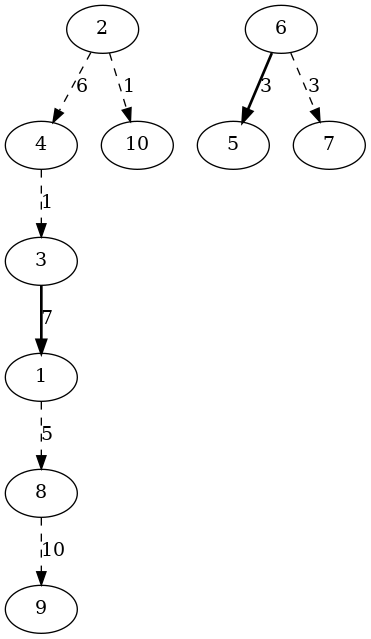
\includegraphics[width=0.35\textwidth]{img/visualisations/test2/cut.png} & 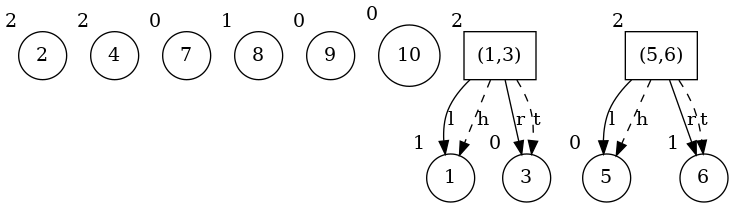
\includegraphics[width=0.7\textwidth]{img/visualisations/test2/icut.png} \\
  Actual tree & Internal tree \\
\end{tabular}
\caption{After \texttt{cut(2)} on tree in Figure \ref{fig:10}}
\label{fig:12}
\end{figure}

\begin{figure}[H]
\centering
\begin{tabular}{cc}
  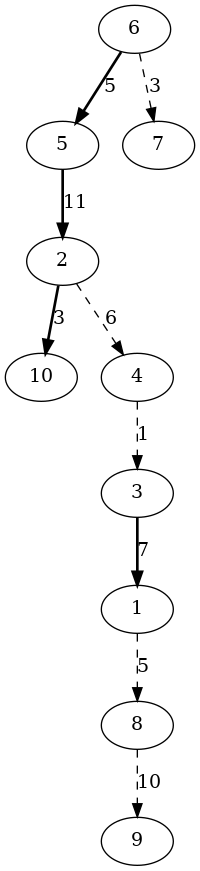
\includegraphics[width=0.25\textwidth]{img/visualisations/test2/update.png} & 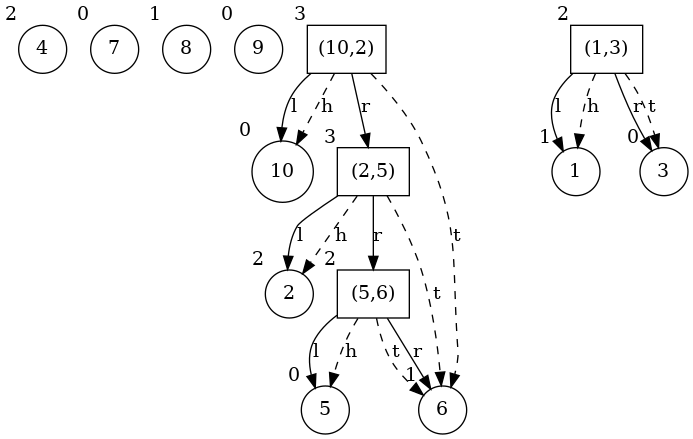
\includegraphics[width=0.75\textwidth]{img/visualisations/test2/iupdate.png} \\
  Actual tree & Internal tree \\
\end{tabular}
\caption{After \texttt{update(10, 2)} on tree in Figure \ref{fig:10}}
\label{fig:13}
\end{figure}

We also note that some of the remaining functions: \texttt{parent}, \texttt{root}, \texttt{cost}, \texttt{mincost}; do potentially modify the bold and dashed paths. We leave the reader to predict and test these changes.

Moreover, we provide the resulting value of the following operations on the tree in Figure \ref{fig:10}:
\begin{itemize}
    \item \texttt{parent(4)} = node 2
    \item \texttt{root(4)} = node 6
    \item \texttt{cost(4)} = 6
    \item \texttt{mincost(4)} = node 5
\end{itemize}

\pagebreak

\section{Understanding Network Flow}

The maximum flow of a network, i.e., given the capacities of various connections, is the maximum amount of flow that can be sent from a source to a sink without exceeding the capacity of any connections.

Dinit’s algorithm generates a level graph which only keeps edges that take us closer to the sink. If no path to a sink is found in generating a level graph, we stop. With the level graph made, we now search for paths to the sink and send flow across it. When considering the paths, we can also traverse an edge in reverse if there is already flow going through it in the forward direction. We keep searching for paths and sending flow until no more paths can be found. This is a blocking flow. Once we reach this state, we generate a new level graph and repeat the process.

Dinit’s algorithm generates at most \(n\) blocking flows. A normal approach takes \(O(nm)\) time to evaluate each of these blocking flows, thus giving an overall time complexity of \(O(n^2m)\) for the max flow problem. However, using dynamic trees, we can reduce the time to \(O(nm\log n)\). (Algorithm steps provided in the paper)

\pagebreak

\section{Analysis}
We start our analysis with a comparison of our unoptimized Dynamic Tree (with a naive implementation of \texttt{construct} and \texttt{split}) and the optimized Dynamic Tree (making use of locally biased binary trees).

We consider the following sequence of \(2n-1\) operations on \(n\) nodes:
\[
\texttt{link(1, 2, 1), link(2, 3, 1), \ldots, link(n-1, n, 1)}
\]
\[
\texttt{cut(1), cut(2), \ldots, cut(n)}
\]

When we compare the performance of the two data structures, we see in Figure \ref{fig:14} that the execution time for the unoptimized data structure rises rapidly. We conjecture its performance to be \(O(n^2)\). Whereas, the theoretical complexity of the optimized Dynamic Tree is \(O(n \log n)\). Our results seem to confirm this.

\begin{figure}[H]
    \centering
    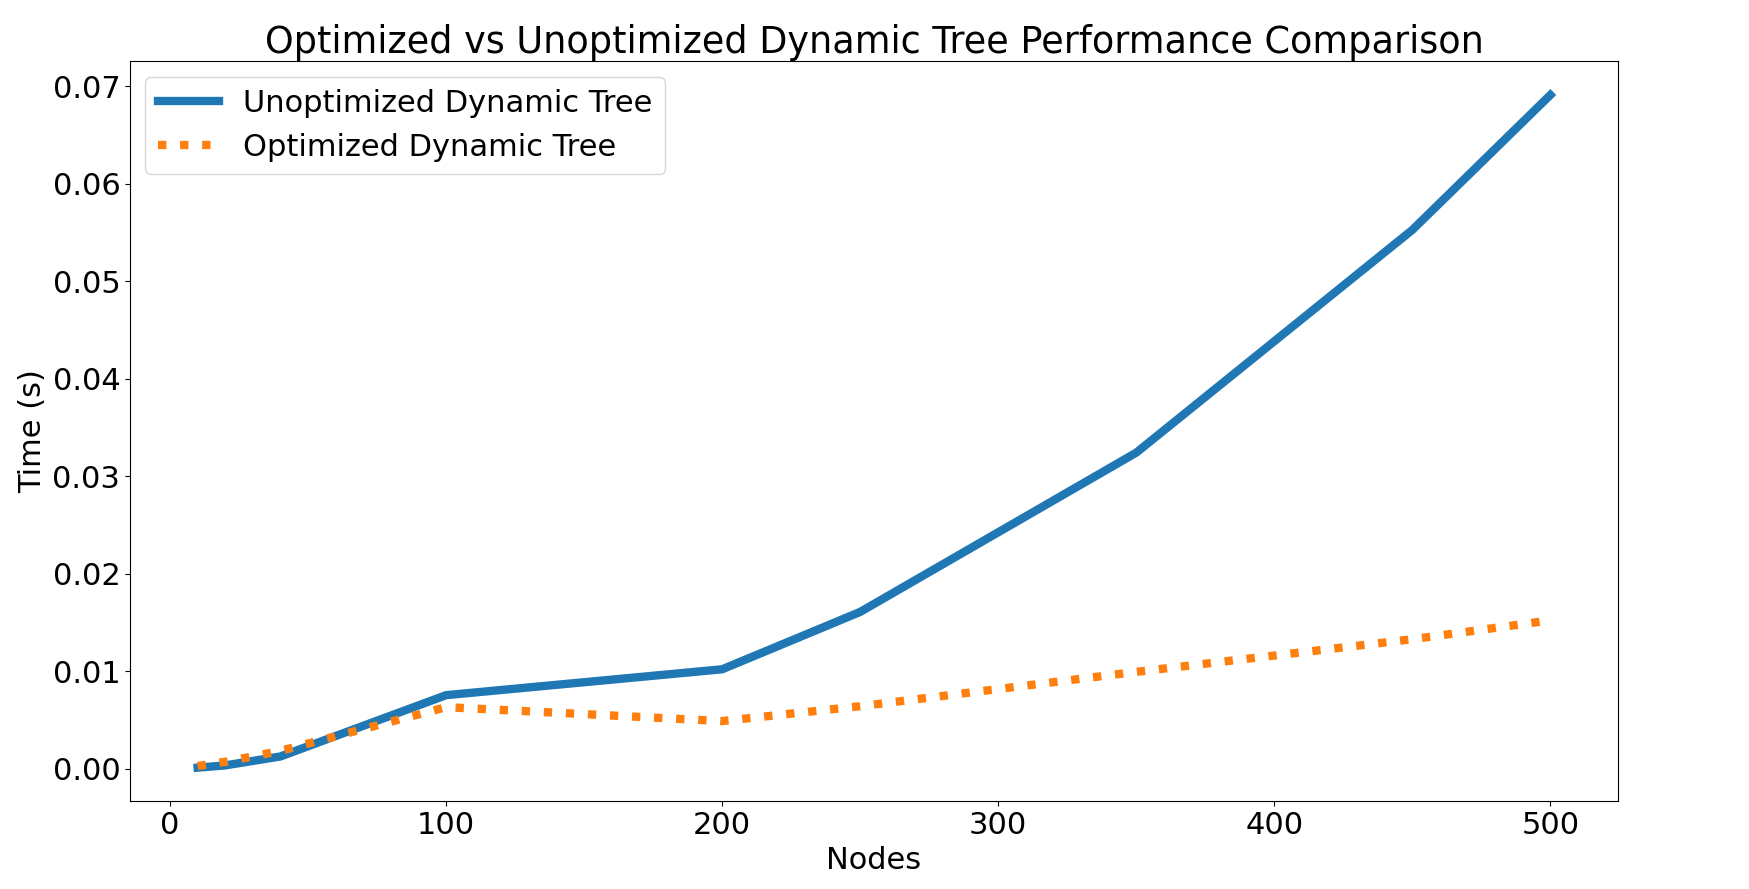
\includegraphics[width=0.9\textwidth]{img/analysis/optim-result.png}
    \caption{The effect of an expose operation.}
    \label{fig:14}
\end{figure}

Now we come to the evaluation of Dynamic Trees for the max flow problem. We generate graphs of \(n\) nodes with random edges, i.e., each possible edge has a specified probability of being present in our graph (in our examples 2\% (Fig. \ref{fig:15}) and 30\% (Fig. \ref{fig:16})) along with a random capacity between 1 and \(n\).

We run the following max flow algorithms:
\begin{itemize}
    \item Ford-Fulkerson - \(O(m^2n)\) - taken from GeeksforGeeks \cite{gg_ff}
    \item Dinit’s max flow algorithm - \(O(n^2m)\) - taken from GeeksforGeeks \cite{gg_dinit}
    \item Dinit’s max flow algorithm (using unoptimized Dynamic Trees) - \(O(n^2m)\) in the worst case
    \item Dinit’s max flow algorithm (using optimized Dynamic Trees) - \(O(nm \log n)\)
\end{itemize}

\begin{figure}[H]
    \centering
    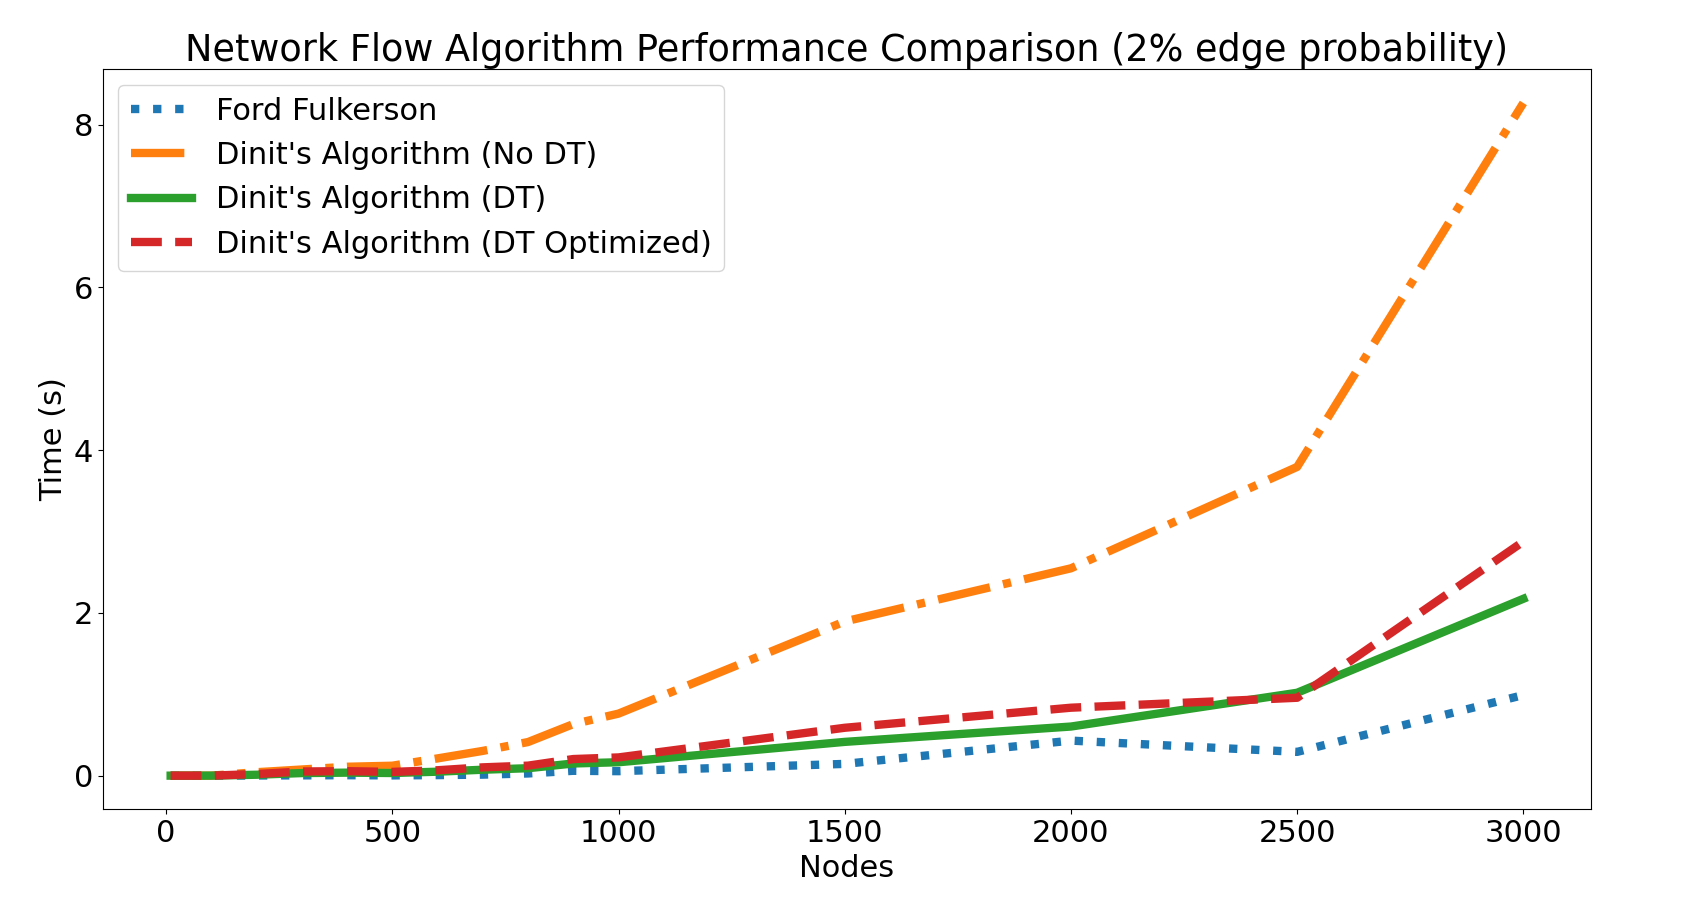
\includegraphics[width=0.9\textwidth]{img/analysis/2-result.png}
    \caption{Network flow algorithm comparison for edge density 2\%.}
    \label{fig:15}
\end{figure}

\begin{figure}[H]
    \centering
    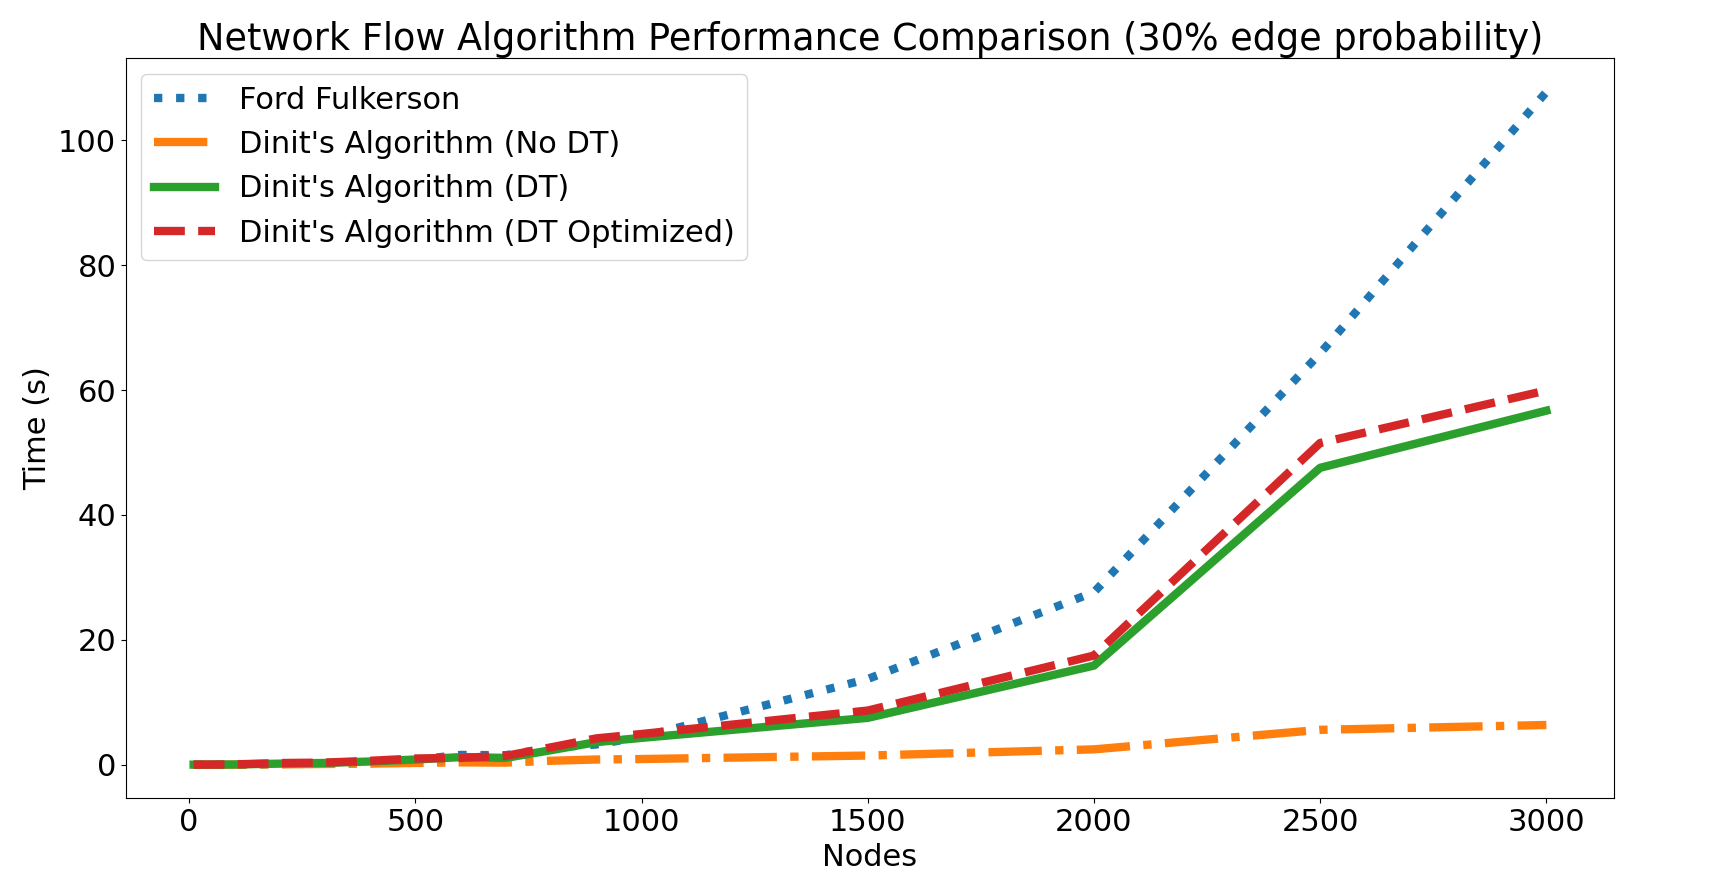
\includegraphics[width=0.9\textwidth]{img/analysis/30-result.png}
    \caption{Network flow algorithm comparison for edge density 30\%.}
    \label{fig:16}
\end{figure}

Note that the calculated values for max flow for all four implementations are tested to match, thereby confirming the validity of the Dynamic Tree and the algorithm's implementation.

Our results have three key insights:
\begin{enumerate}
    \item The two variants of the Dynamic Trees have minimal difference in execution. In fact, the unoptimized data structure often outperforms the optimized one. We believe this to be due to the randomization in the generation of the input graph which carries out an implicit balancing of the internal tree.
    \item For fewer numbers of edges (Fig. \ref{fig:15}), where the impact on execution is largely from the number of nodes, Dinit’s max flow using Dynamic Trees notably outperforms the general Dinit’s max flow algorithm. Ford-Fulkerson performs best as it has the smallest dependency on the number of nodes for execution.
    \item For a larger number of edges (Figure \ref{fig:16}), where the impact on execution is largely due to the number of edges, Dinit’s max flow using Dynamic Trees struggles to compete with the general Dinit’s max flow algorithm. Perhaps this is due to large constant costs in the Dynamic Tree. Moreover, we see that our Dynamic Tree implementation does outperform Ford-Fulkerson, thus confirming that our implementation isn’t just a worse version of Ford-Fulkerson.
\end{enumerate}

The discrepancy in the last result in the Dynamic Tree implementation versus the general Dinit’s algorithm may be because the number of edges is not fixed but rather is a function of the number of vertices. We note that the expected number of edges is $n^2 \times prob\_edge$.

Regardless, we conclude that the Dynamic Trees do seem to be implementing a version of Dinit’s flow, as can be seen by their ability to outperform the Ford-Fulkerson algorithm for a large number of edges. Moreover, it also seems to be optimizing on Dinit’s as it outperforms it when edge density is low.

\pagebreak

\section{Conclusion}
Overall, Sleator and Tarjan’s approach to the Dynamic Trees problem is highly creative, making use of many clever tricks and optimizations. Implementing the data structure was a significant challenge, especially when venturing into ideas that weren’t clearly detailed within the paper. Nonetheless, we have managed to implement this data structure and visualize its operations.

Moreover, we were seemingly able to verify the results and bounds that Sleator and Tarjan had theoretically proven through empirical testing. The optimized data structure did seemingly perform \(O(m)\) operations in \(O(m \log n)\) time as opposed to the unoptimized version. And the network flow algorithm was not only yielding accurate results but was also able to compete against the generic version of Dinit’s for sparse graphs and against Ford-Fulkerson for dense graphs.

We do note that one major limitation of our work is that for testing network flow, the use of a randomized graph may have skewed some of the results, considering how it had enabled the unoptimized data structure to compete with the optimized one. Moreover, our system of using edge densities impacts analysis focusing on the effect of the number of nodes.

For future work, we encourage readers to create their own, more holistic test cases for the data structure. We also encourage readers to carry out a theoretical analysis of our setup, where the number of edges was directly related to the number of nodes, to determine if that was the cause of discrepancy in the analysis results.

\pagebreak

\section{Appendix}
\begin{enumerate}
\item \textbf{\textit{Revised explanation for \texttt{pmincost(p)} (errors in bold—comments in [ ])}}: \\
Starting from \(p\), which is the root of a binary tree, proceed downward in the tree, keeping track of reversal states, until finding the node \(u\) last in symmetric order such that \texttt{grosscost(u)} = \textbf{grossmin(p)} [because that means the edge represented by \(u\) has the least cost in the path]. This can be done by initializing \(u\) to be \(p\) and repeating the following step until \(u\) has \texttt{netcost} zero and its right child is either external or has positive \texttt{netmin}: if the right child of \(u\) is internal and has \textbf{netmin} zero [as \texttt{netmin} allows me to check if the least cost edge is in this subtree or not], replace \(u\) by its right child; otherwise if \(u\) has positive \texttt{netcost}, replace \(u\) by its left child.

\item \textbf{\textit{Revised pseudocode for \texttt{expose} (errors in bold)}}:
\begin{verbatim}
function expose(v):
    path p, q, r; real x, y;
    [q,r,x,y] := split(v)
    if q != null ->
        dparent(tail(q)), dcost(tail(q)) := v, x;
        wt(v) := wt(v) + wt(q)
    fi;
\end{verbatim}
\-\hspace{0.9cm}\textbf{rank(v) = log(wt(v));}
\begin{verbatim}
    if r = null -> p := path(v)
     | r != null -> p := concatenate(path(v), r, y)
    fi;
    do dparent(tail(p)) != null -> p := splice(p) od;
    return p
end expose;
\end{verbatim}

\item \textbf{\textit{GitHub Repository}}: \href{https://github.com/Musab1Blaser/DynamicTrees_NF}{DynamicTree\_NF}
\end{enumerate}

\pagebreak

\bibliographystyle{ieeetr}
\bibliography{bibliography}  % need to put bibtex references in references.bib 
\end{document}